\documentclass[a4paper,11pt,fleqn,dvipsnames,oneside,openright]{memoir} 	% Openright aabner kapitler paa hoejresider (openany begge)

%%%% PACKAGES %%%%

% ¤¤ Oversaettelse og tegnsaetning ¤¤ %
\usepackage[utf8]{inputenc}					% Input-indkodning af tegnsaet (UTF8)
\usepackage[danish]{babel}					% Dokumentets sprog
\usepackage[T1]{fontenc}					% Output-indkodning af tegnsaet (T1)
\usepackage{ragged2e,anyfontsize}			% Justering af elementer
\usepackage{fixltx2e}						% Retter forskellige fejl i LaTeX-kernen
																			
% ¤¤ Figurer og tabeller (floats) ¤¤ %
\usepackage{graphicx} 						% Haandtering af eksterne billeder (JPG, PNG, EPS, PDF)

\usepackage{subfig}

%\usepackage{eso-pic}						% Tilfoej billedekommandoer paa hver side
%\usepackage{wrapfig}						% Indsaettelse af figurer omsvoebt af tekst. \begin{wrapfigure}{Placering}{Stoerrelse}
\usepackage[space]{grffile}					% Bør gøre det muligt at have mellemrum i filnavne.
\usepackage{multirow}                		% Fletning af raekker og kolonner (\multicolumn og \multirow)
\usepackage{multicol}         	        	% Muliggoer output i spalter
\usepackage{rotating}						% Rotation af tekst med \begin{sideways}...\end{sideways}
\usepackage{colortbl} 						% Farver i tabeller (fx \columncolor og \rowcolor)
\usepackage[usenames,dvipsnames]{xcolor}	% Definer farver med \definecolor. Se mere: http://en.wikibooks.org/wiki/LaTeX/Colors
%\usepackage{flafter}						% Soerger for at floats ikke optraeder i teksten foer deres reference
\let\newfloat\relax 						% Justering mellem float-pakken og memoir
\usepackage{float}							% Muliggoer eksakt placering af floats, f.eks. \begin{figure}[H]
\setlength{\heavyrulewidth}{0.15em}			% Sætter \toprule og \bottomrule til fast størrelse (0.08 er default)
%\setlength{\lightrulewidth}{0.05em}		% Sætter \midrule til fast størrelse (0.05 er default)
\usepackage{array}							% Bruges i forbindelse med \newcolumntype-command under egne commands
\usepackage{pdfpages}						% Bruges så der kan indsættes pdf, som sider (forside for eksempel)
\usepackage{wrapfig}
\usepackage[section]{placeins}				% Indsætter en border så billeder bliver placeret inden for den section de er indsat
\usepackage{lastpage}						% Anvendes til at se total antal sider

% ¤¤ Matematik mm. ¤¤
\usepackage{amsmath,amssymb,stmaryrd} 		% Avancerede matematik-udvidelser
\usepackage{mathtools}						% Andre matematik- og tegnudvidelser
\usepackage{textcomp}                 		% Symbol-udvidelser (f.eks. promille-tegn med \textperthousand )
\usepackage{rsphrase}						% Kemi-pakke til RS-saetninger, f.eks. \rsphrase{R1}
\usepackage[version=3]{mhchem} 				% Kemi-pakke til flot og let notation af formler, f.eks. \ce{Fe2O3}
\usepackage{siunitx}						% Flot og konsistent praesentation af tal og enheder med \si{enhed} og \SI{tal}{enhed}
\sisetup{locale=DE}							% Opsaetning af \SI (DE for komma som decimalseparator) 

% ¤¤ Referencer og kilder ¤¤ %
\usepackage[danish]{varioref}				% Muliggoer bl.a. krydshenvisninger med sidetal (\vref)
\usepackage{natbib}							% Udvidelse med naturvidenskabelige citationsmodeller
\usepackage{xr-hyper}							% Referencer til eksternt dokument med \externaldocument{<NAVN>}
\externaldocument[DokRap-]{../Dokumentationsrapport/Dokumentationsrapport}	% Muliggør eksterne referencer til dokumentationsrapporten
%\usepackage{glossaries}					% Terminologi- eller symbolliste (se mere i Daleifs Latex-bog)



% ¤¤ Misc. ¤¤ %
\usepackage{lipsum}							% Dummy text \lipsum[..]
\usepackage[shortlabels]{enumitem}			% Muliggoer enkelt konfiguration af lister
\usepackage{pdfpages}						% Goer det muligt at inkludere pdf-dokumenter med kommandoen \includepdf[pages={x-y}]{fil.pdf}	
\pdfoptionpdfminorversion=6					% Muliggoer inkludering af pdf dokumenter, af version 1.6 og hoejere
\pretolerance=2500 							% Justering af afstand mellem ord (hoejt tal, mindre orddeling og mere luft mellem ord)

% Kommentarer og rettelser med \fxnote. Med 'final' i stedet for 'draft' udloeser hver note en error i den faerdige rapport.
\usepackage[footnote,draft,danish,silent,nomargin]{fixme}	

%lists
\usepackage{listings}	


%%%% CUSTOM SETTINGS %%%%

% ¤¤ Marginer ¤¤ %
\setlrmarginsandblock{3.5cm}{2.5cm}{*}		% \setlrmarginsandblock{Indbinding}{Kant}{Ratio}
\setulmarginsandblock{2.5cm}{3.0cm}{*}		% \setulmarginsandblock{Top}{Bund}{Ratio}
\checkandfixthelayout 						% Oversaetter vaerdier til brug for andre pakker

%	¤¤ Afsnitsformatering ¤¤ %
\setlength{\parindent}{0mm}           		% Stoerrelse af indryk
\setlength{\parskip}{3mm}          			% Afstand mellem afsnit ved brug af double Enter
\linespread{1,1}							% Linie afstand
\newcommand{\tab}{\hspace*{2em}}			% ved \tab{} indrykkes det i klammerne ind
\usepackage{titlesec}							%Muliiggøre ændring af sections i alle lag
\titleformat*{\section}{\LARGE\bfseries\color{NavyBlue}}		%section = størst
\titleformat*{\subsection}{\Large\bfseries\color{RoyalBlue}}		%sub og subsub har samme størrelse
\titleformat*{\subsubsection}{\Large\bfseries}
\titleformat*{\paragraph}{\large\bfseries}		%Benyttes umiddelbart ikke
\titleformat*{\subparagraph}{\large\bfseries}	%Benyttes umiddelbart ikke

% ¤¤ Litteraturlisten ¤¤ %
\bibpunct[,]{[}{]}{;}{a}{,}{,} 				% Definerer de 6 parametre ved Harvard henvisning (bl.a. parantestype og seperatortegn)
\bibliographystyle{bibtex/harvard}			% Udseende af litteraturlisten.

% ¤¤ Indholdsfortegnelse ¤¤ %
\setsecnumdepth{subsubsection}		 		% Dybden af nummerede overkrifter (part/chapter/section/subsection)
\maxsecnumdepth{subsection}					% Dokumentklassens graense for nummereringsdybde
\settocdepth{subsubsection} 				% Dybden af indholdsfortegnelsen

% ¤¤ Lister ¤¤ %
\setlist{
  topsep=-5pt,								% Vertikal afstand mellem tekst og listen	Default: 0
  itemsep=-1ex,								% Vertikal afstand mellem items
} 

% ¤¤ Visuelle referencer ¤¤ %
\usepackage[colorlinks]{hyperref}			% Danner klikbare referencer (hyperlinks) i dokumentet.
\hypersetup{colorlinks = true,				% Opsaetning af farvede hyperlinks (interne links, citeringer og URL)
    linkcolor = black,
    citecolor = black,
    urlcolor = black
}

% ¤¤ Opsaetning af figur- og tabeltekst ¤¤ %
\usepackage{caption}
\captionnamefont{\small\bfseries\itshape}	% Opsaetning af tekstdelen ('Figur' eller 'Tabel')
\captiontitlefont{\small}					% Opsaetning af nummerering
\captiondelim{. }							% Seperator mellem nummerering og figurtekst
\hangcaption								% Venstrejusterer flere-liniers figurtekst under hinanden
\captionsetup{width=\linewidth,labelfont={bf,it}}
\setlength{\abovecaptionskip}{5pt}			% Afstand over figurteksten
\setlength{\belowcaptionskip}{-12pt}		% Afstand under figurteksten
		
% ¤¤ Navngivning ¤¤ %
\addto\captionsdanish{
	\renewcommand\appendixname{Appendiks}
	\renewcommand\contentsname{Indholdsfortegnelse}	
	\renewcommand\appendixpagename{Appendiks}
	\renewcommand\appendixtocname{Appendiks}
	\renewcommand\cftchaptername{\chaptername~}				% Skriver "Kapitel" foran kapitlerne i indholdsfortegnelsen
	\renewcommand\cftappendixname{\appendixname~}			% Skriver "Appendiks" foran appendiks i indholdsfortegnelsen
}

% ¤¤ Kapiteludssende ¤¤ %
\definecolor{chapnumcolor}{RGB}{23,54,93}		% Definerer en farve til brug til kapiteludseende
\definecolor{chapfontcolor}{RGB}{29,69,118}
\newif\ifchapternonum

\makechapterstyle{jenor}{					% Definerer kapiteludseende frem til ...
  \renewcommand\beforechapskip{0pt}
  \renewcommand\printchaptername{}
  \renewcommand\printchapternum{}
  \renewcommand\printchapternonum{\chapternonumtrue}
  \renewcommand\chaptitlefont{\fontfamily{pbk}\fontseries{db}\fontshape{n}\fontsize{25}{35}\selectfont\raggedleft\color{chapfontcolor}}
  \renewcommand\chapnumfont{\fontfamily{pbk}\fontseries{m}\fontshape{n}\fontsize{1in}{0in}\selectfont\color{chapnumcolor}}
  \renewcommand\printchaptertitle[1]{%
    \noindent
    \ifchapternonum
    \begin{tabularx}{\textwidth}{X}
    {\let\\\newline\chaptitlefont ##1\par} 
    \end{tabularx}
    \par\vskip-2.5mm\hrule
    \else
    \begin{tabularx}{\textwidth}{Xl}
    {\parbox[b]{\linewidth}{\chaptitlefont ##1}} & \raisebox{-15pt}{\chapnumfont \thechapter}
    \end{tabularx}
    \par\vskip2mm\hrule
    \fi
  }
}											% ... her

\chapterstyle{jenor}						% Valg af kapiteludseende - Google 'memoir chapter styles' for alternativer

% ¤¤ Sidehoved ¤¤ %

\makepagestyle{AAU}							% Definerer sidehoved og sidefod udseende frem til ...
\makepsmarks{AAU}{%
	\createmark{chapter}{left}{shownumber}{}{. \ }
	\createmark{section}{right}{shownumber}{}{. \ }
	\createplainmark{toc}{both}{\contentsname}
	\createplainmark{lof}{both}{\listfigurename}
	\createplainmark{lot}{both}{\listtablename}
	\createplainmark{bib}{both}{\bibname}
	\createplainmark{index}{both}{\indexname}
	\createplainmark{glossary}{both}{\glossaryname}
}
\nouppercaseheads											% Ingen Caps oenskes

\makeevenhead{AAU}{Test}{}{\leftmark}					% Definerer lige siders sidehoved (\makeevenhead{Navn}{Venstre}{Center}{Hoejre})
\makeoddhead{AAU}{\rightmark}{}{Ingeniørhøjskolen, Aarhus Universitet}		% Definerer ulige siders sidehoved (\makeoddhead{Navn}{Venstre}{Center}{Hoejre})
\makeevenfoot{AAU}{\thepage}{}{}							% Definerer lige siders sidefod (\makeevenfoot{Navn}{Venstre}{Center}{Hoejre})
\makeoddfoot{AAU}{}{}{\thepage}								% Definerer ulige siders sidefod (\makeoddfoot{Navn}{Venstre}{Center}{Hoejre})
\makeheadrule{AAU}{\textwidth}{0.5pt}						% Tilfoejer en streg under sidehovedets indhold
\makefootrule{AAU}{\textwidth}{0.5pt}{1mm}					% Tilfoejer en streg under sidefodens indhold

\copypagestyle{AAUchap}{AAU}								% Sidehoved for kapitelsider defineres som standardsider, men med blank sidehoved
\makeoddhead{AAUchap}{}{}{}
\makeevenhead{AAUchap}{}{}{}
\makeheadrule{AAUchap}{\textwidth}{0pt}
\aliaspagestyle{chapter}{AAUchap}							% Den ny style vaelges til at gaelde for chapters
															% ... her
															
\pagestyle{AAU}												% Valg af sidehoved og sidefod



% Opsætning af source code import
% \lstinputlisting{sti../navn.endelse}
\lstset{
  language=C,                		% choose the language of the code
  numbers=left,                   	% where to put the line-numbers
  stepnumber=1,                   	% the step between two line-numbers.        
  numbersep=5pt,                  	% how far the line-numbers are from the code
  backgroundcolor=\color{white},  	% choose the background color. You must add \usepackage{color}
  showspaces=false,               	% show spaces adding particular underscores
  showstringspaces=false,         	% underline spaces within strings
  showtabs=false,                 	% show tabs within strings adding particular underscores
  tabsize=2,                      	% sets default tabsize to 2 spaces
  captionpos=b,                   	% sets the caption-position to bottom
  breaklines=true,                	% sets automatic line breaking
  breakatwhitespace=true,         	% sets if automatic breaks should only happen at whitespace
  title=\lstname,                 	% show the filename of files included with \lstinputlisting;
  emph={ uint8, uint16, void }, emphstyle={\color{blue}}	% tilføj variabel hvis de skal markeres blå
}






%%%% CUSTOM COMMANDS %%%%

% ¤¤ Billede hack ¤¤ %
\newcommand{\figur}[4]{
		\begin{figure}[H] \centering
			\includegraphics[width=#1\textwidth]{Billeder/#2}
			\caption{#3}\label{#4}
		\end{figure} 
}


% ¤¤ Venstre orienterer al tekst i p{Ycm} ¤¤ %
\newcolumntype{x}[1]{%
>{\raggedright\hspace{0pt}}p{#1}}

% ¤¤ Newline til x{} ¤¤ %
% \\ virker åbenbart ikke når man selv laver en columntype... :(
\newcommand{\tn}{\tabularnewline}

% ¤¤ Newline til x{} ¤¤ %
% \\ virker åbenbart ikke når man selv laver en columntype... :(
\newcommand{\tnhl}{\tabularnewline\hline}



% ¤¤ Nyt environment til indsættelse af A3-størrelse figurer
\newenvironment{A3Figure}
{
	\cleardoublepage
	\pageaiii
	\setlength{\pdfpagewidth}{\paperheight} % Change the pdf page to A3 height
	\setlength{\pdfpageheight}{\paperwidth} % Change the pdf height to A3 width
	\setlength{\textwidth}{\paperheight - \the\spinemargin-\the\foremargin} % Change the textwidth
}
{
	\cleardoublepage	
}

% funktions beskrivelse void argument%
\newcommand{\funcDescrip}[2]{
\textbf{{\color{blue} #1} #2({\color{blue} void})} \\
}

% funktions beskrivelse 1 argument%
\newcommand{\funcDescripOne}[4]{
\textbf{{\color{blue} #1} #2({\color{blue} #3} #4)} \\
}

% funktions beskrivelse 2 argument%
\newcommand{\funcDescripTwo}[6]{
\textbf{{\color{blue} #1} #2({\color{blue} #3} #4, {\color{blue} #5} #6)} \\
}

% opsætning af funktions tabel %
\newcommand{\funcTabel}[4]{
\begin{tabular}{p{0.2cm}p{3cm}p{11cm}} \hline
	&	\textbf{Description:} 		& 	#1	\\
	&	\textbf{Parameters:} 		& 	#2	\\
	&	\textbf{Return Value:}		& 	#3	\\
	&	\textbf{Side Effects:}		&	#4	\\
\end{tabular}
}


% ¤¤ Units i math-environments ¤¤ %
\newcommand{\mathUnit}[2]{\mathrm{\si{#1}{#2}}}







% ¤¤ Pæn opsætning af titelblad-dele ¤¤ %
% ¤¤ Husk at ændre dato i senere projekter ¤¤ %
\newcommand{\titelblad}[2]{
\begin{tabular}[ht]{x{7cm}x{7cm}}
\textbf{Navn: } #1		&\textbf{Studienummer: } #2	\tn
\textbf{Dato} 2013-05-31	\tn
\multicolumn{2}{l}{\textbf{Underskrift: }\line(1,0){340}}
\end{tabular}
}


% ¤¤ Specielle tegn ¤¤ %
\newcommand{\grader}{^{\circ}\text{C}}   % Grader C, virker kun i math-environments
\newcommand{\gr}{^{\circ}}
\newcommand{\g}{\cdot}		% Gange i math-environments
\newcommand{\grC}{$^{\circ}\mathrm{C}$}		% Grader C, uden for math-environments

%%%% ORDDELING %%%%

\hyphenation{}

%%%Indsat af Søren%%%
\usepackage{listings}
\usepackage{color}
 
\definecolor{dkgreen}{rgb}{0,0.6,0}
\definecolor{gray}{rgb}{0.5,0.5,0.5}
\definecolor{mauve}{rgb}{0.58,0,0.82}
 
\lstset{ %
  language=Octave,                % the language of the code
  basicstyle=\footnotesize,           % the size of the fonts that are used for the code
  numbers=left,                   % where to put the line-numbers
  numberstyle=\tiny\color{gray},  % the style that is used for the line-numbers
  stepnumber=2,                   % the step between two line-numbers. If it's 1, each line 
                                  % will be numbered
  numbersep=5pt,                  % how far the line-numbers are from the code
  backgroundcolor=\color{white},      % choose the background color. You must add \usepackage{color}
  showspaces=false,               % show spaces adding particular underscores
  showstringspaces=false,         % underline spaces within strings
  showtabs=false,                 % show tabs within strings adding particular underscores
  frame=single,                   % adds a frame around the code
  rulecolor=\color{black},        % if not set, the frame-color may be changed on line-breaks within not-black text (e.g. comments (green here))
  tabsize=2,                      % sets default tabsize to 2 spaces
  captionpos=b,                   % sets the caption-position to bottom
  breaklines=true,                % sets automatic line breaking
  breakatwhitespace=false,        % sets if automatic breaks should only happen at whitespace
  title=\lstname,                   % show the filename of files included with \lstinputlisting;
                                  % also try caption instead of title
  keywordstyle=\color{blue},          % keyword style
  commentstyle=\color{dkgreen},       % comment style
  stringstyle=\color{mauve},         % string literal style
  escapeinside={\%*}{*)},            % if you want to add LaTeX within your code
  morekeywords={*,...},              % if you want to add more keywords to the set
  deletekeywords={...}              % if you want to delete keywords from the given language
}											% Preamble 
\raggedbottom													% LaTeX "straekker" ikke teksten

%\includeonly{file1,file2}										% Inkluder kun specifikke filer 

\begin{document}												% Starter
\frontmatter													% Forindhold - nummereres med romertal
\thispagestyle{empty}
\begin{flushright}
\vspace{3cm}

\phantom{hul}

\phantom{hul}

\phantom{hul}

\textsl{\Huge Skeleton Project} \\ \vspace{1cm}

\rule{13cm}{3mm} \\ \vspace{1.5cm}
\vspace{1cm}


\includegraphics[width=0.4\textwidth]{4.Construction/pictures/skeleton-cover.jpg}

\vspace{2cm} 
\textsc{\Large Skeleton Project V1 \\
Group of project \\
Faculty\\
Delivery date\\}
\end{flushright}


%%%% Indholdsfortegnelse (TOC) %%%%
\tableofcontents*												%Indholdsfortegnelsen (kaldet ToC) 

\mainmatter														% Hovedindhold - nummereres fra side 1
\chapter{Systemarkitektur}

\section{Revisionshistorik}
\begin{table}[H]
	\centering
		\begin{tabular}{|p{2 cm}|p{2 cm}|p{3 cm}|p{6 cm}|} 
		\hline
			\textbf{Rev. Nr} & \textbf{Dato}		& \textbf{Initialer} 	& \textbf{Ændring} \\ \hline
			1.0 	& & &  \\ \hline
			1.1 	& & &	\\ \hline
		\end{tabular}
	\caption{Revisionshistorik}
	%\label{tab:TC1}
\end{table}

\vspace{1.5cm}

\section{Ordforklaring}
\begin{table}[H]
	\centering
		\begin{tabular}{|p{2.5cm}|p{4.5 cm}|p{6.5 cm}|} 
		\hline
			\textbf{Forkortelse} & \textbf{Betydning} & \textbf{Forklaring} \\ \hline
			 &  &  \\ \hline
			 &  & \\ \hline
		\end{tabular}
	\caption{Ordforklaring}
	%\label{tab:TC1}
\end{table}

\vspace{2cm}

\section{Indledning}
Dette kapitel beskriver hvilke enheder systemet består af samt grænseflader mellem
enhederne. Til at beskrive hardware og tilhørende grænseflader benyttes SysML diagrammer, mens software og tilhørende grænseflader beskrives med UML diagrammer.
\section{Indledning}

I projektforløbet er der løbende blevet udført test. Indledningsvis udføres enhedstest i takt med nye enheder udvikles, senere laves integrationstest der tester kommunikation og samarbejde mellem flere enheder og til sidst udføres accepttest, der bruges til at teste det samlede system. Nedenfor beskrivelses de forskellige tests:


\subsection{Enhedstest} 
\vspace{-0.5cm}
Enhedstest er en testmetode der benyttes til at isolere og teste systemets enkelte enheder. Enhedstest udføres løbende i takt med nye enheder udvikles. Testene udarbejdes for at sikre kvalitet, funktionalitet og grænseflader af de nyudviklede enheder. 

Hovedformålet med enhedstest er at teste tidligt i projektforløbet for at opdage eventuelle fejl og mangler. Hvilket i sidste ende sparer gruppen for meget tid og besvær, da fejl og mangler er svære og mere tidskrævende at rette sent i et projektforløb.

Figur \ref{fig:test_forlob} illustrerer hvordan mange fejl kan findes ved brug af enhedstest. Fejl der ellers "først" var blevet fundet når systemets enheder blev koblet sammen.
\vspace{-0.4cm}
\begin{figure}[H]
	\centering
	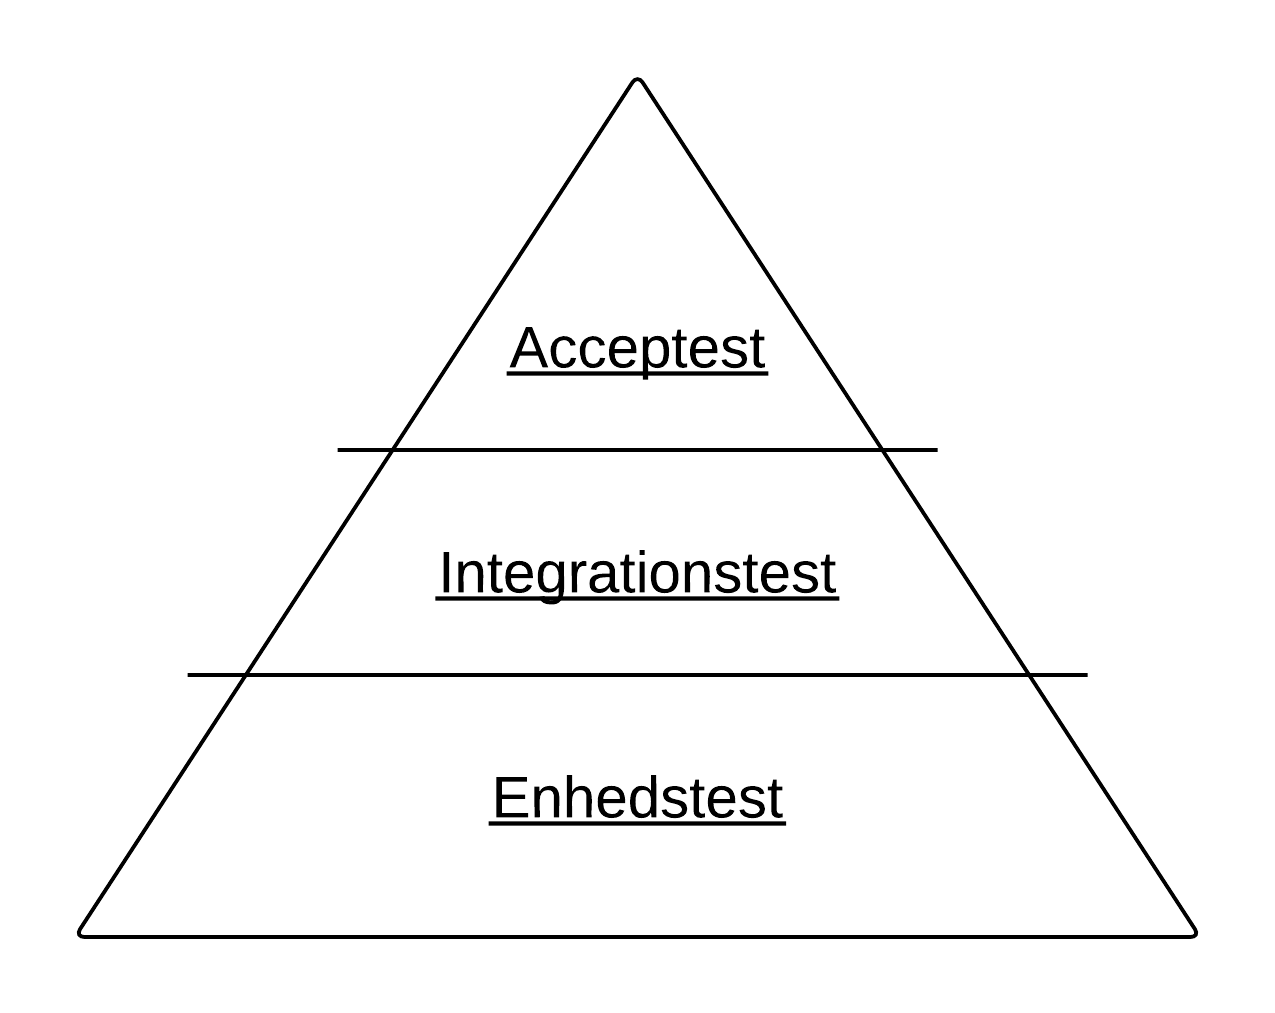
\includegraphics[width=0.5\textwidth]{Billeder/Test/forlob.png}
	\vspace{-0.4cm}
	\caption{Mængde af fejl fundet ved test}
	\label{fig:test_forlob}
\end{figure}

\vspace{0.5cm}

Enhedstest bygges som regel op efter AAA-modellen\footnote{http://c2.com/cgi/wiki?ArrangeActAssert}.\\ 
\textbf{A}rrange: Opsætning af input til test og håndtering af afhængigheder. \\
\textbf{A}ct: Hardware/software enhed under test stimuleres. \\
\textbf{A}ssert: Der kigges på output og det afgøres om testen er succesfuld eller ej.

På  figur \ref{fig:aaa} ses et eksempel på software test efter AAA modellen. I testen bliver der testet om den korrekte metode bliver kaldt når bruger prøver at logge in på webapplikationen. 

\begin{figure}[H]
	\centering
	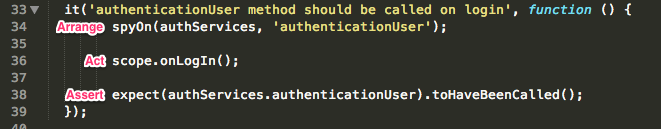
\includegraphics[width=0.75\textwidth]{Billeder/Test/aaa.png}
	\caption{AAA eksempel}
	\label{fig:aaa}
\end{figure}

\newpage

\subsection{Integrationstest} 
Integrationstest bruges til at teste kobling mellem to eller flere enheder. Integrationstest bruges til at kontrollere om enhederne under test kan kommunikere og arbejde sammen. 

Integrationstest af hardware og tilhørende software klasser er udført efter Collaboration modellen, mens software til server og webapplikation er integrationstestet efter metoderne buttom-up, top-down og collaboration. \\

\vspace{-0.4cm}

\textbf{Collaboration}\\
Når der testes efter collaboration samles en række enheder. Inden sammenkobling udgør hver enhed en lille klump funktionalitet, men tilsammen udgør enhederne en væsentlig del af systemts samlede funktionalitet.
På figur \ref{fig:Collaboration} illustreres et eksempel på collaboration.

\vspace{-5pt}
%kommentar
\begin{figure}[H]
	\centering
	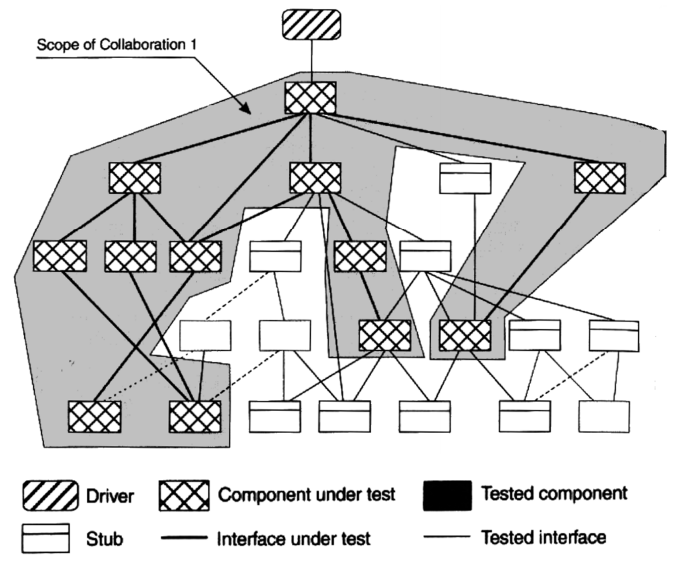
\includegraphics[width=0.6\textwidth]{Billeder/Test/collaboration.png}
	\vspace{-5pt}
	\caption{Collaboration}
	\label{fig:Collaboration}
\end{figure}


\textbf{Button-Up}\\
På figur \ref{fig:Buttom_up} ses et eksempel på buttom up testing. Figuren viser hvordan systemets mest grundlæggende klasser er først testet og derefter bliver der testet op igennem systemet. 

%kommentar
\begin{figure}[H]
	\centering
	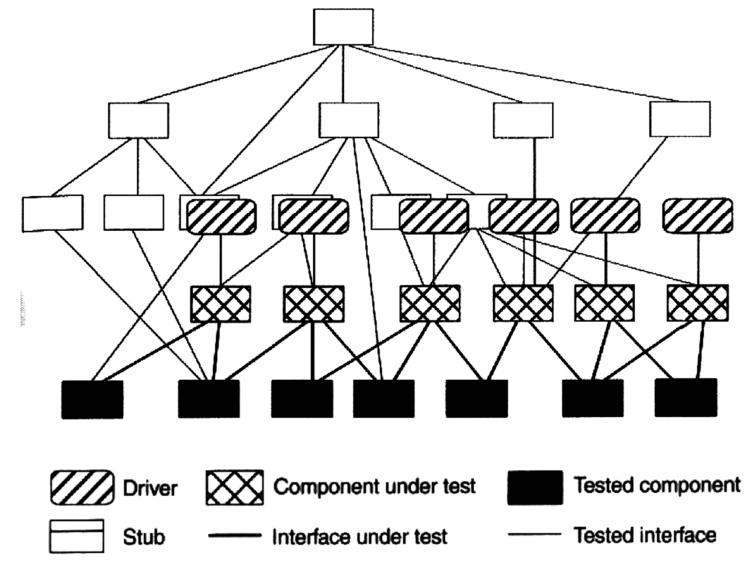
\includegraphics[width=0.6\textwidth]{Billeder/Test/buttom-up.png}
	\vspace{-5pt}
	\caption{Buttom up}
	\label{fig:Buttom_up}
\end{figure}

\newpage

\textbf{Top-Down}\\
På figur \ref{fig:Top_down} ses et eksempel på top down testing. Figuren vises hvordan systemets top klasser er testet først og derefter testet ned igennem klasserne.

%kommentar
\begin{figure}[H]
	\centering
	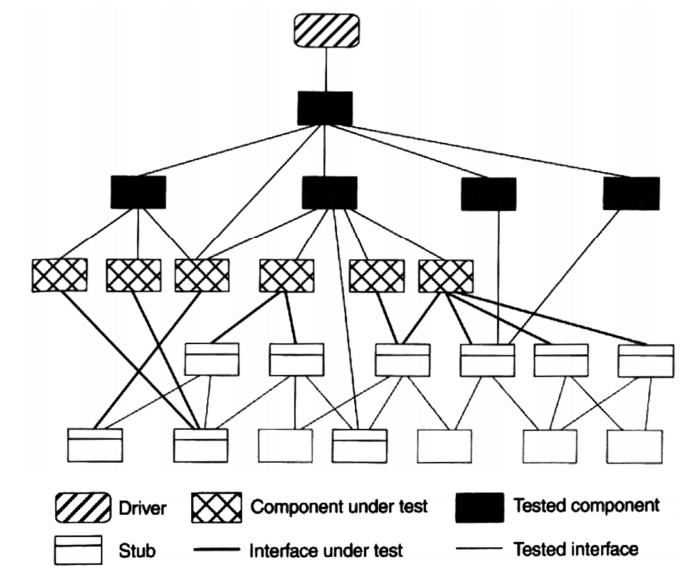
\includegraphics[width=0.65\textwidth]{Billeder/Test/top-down.png}
	\vspace{-5pt}
	\caption{Top down}
	\label{fig:Top_down}
\end{figure}

\vspace{1.5cm}

\subsection{Accepttest} 
Accepttesten er en todelt test der tester systemet som helhed. 
Først udføres accepttest af funktionelle krav og dernæst testes ikke-funktionelle krav.
Accepttest af funktionelle krav foregår via en gennemgang af use cases, som bruges til at kontrollere systemets funktionalitet. Ikke-funktionelle krav bruges til at teste systemspecifikationer.  

\section{Drone}

Dronen der skal anvendes vælges på baggrund af analysen beskrevet i denne sektion. 

I dokumentet søges information og afklaring af følgende punkter:
\begin{itemize}
	\item Pris.
	\item Løftekapacitet. 
	\item Tilgængelighed af reservedele. 
	\item Open source kode til regulering (motorstyring)
\end{itemize}

\vspace{0.5cm}

Ud fra kriterierne stod valget af drone mellem to forskellige quadrocopterer: 
3DR – Quadrocopter:  Det amerikanske firma 3D Robotics udvikler droner i forskellige størrelser. Quadrocopterer fra 3DR kan enten købes færdige eller som ”byg selv” projekter. Det bedst egnede til projektet er et ”byg selv” kit der hedder DIY Quad Kit\footnote{https://store.3drobotics.com/products/diy-quad-kit}. 

Ved køb af kittet fås 4x 10 x 4.7 propeller, 20 Amp ESC’er (motor kontrol) og motorer der maksimalt kan rotere 850 gange pr min / volt.  Desuden medfølger et motorstyringsmodul og styringssoftwaren er open source. Den samlede pris for DIY Quad kittet ligger på 549 USD. Det bemærkes, at batteri / batterier til quadrocopteren skal købes separat.

AeroQuad: Det Amerikanske firma AeroQuad har lavet quadrocopteren AeroQuad Cyclone ARF. Aeroquad'en\footnote{http://www.aeroquadstore.com/AeroQuad\textunderscore Cyclone\textunderscore ARF\textunderscore Kit\textunderscore p/aqarf-001.htm} er en kraftig quadrocopter med 12” propeller og motorer der yder 950 Kv ( 950 rpm/V). Til motorstyring følger open source styringssoftware samt fire 20 amperes ESC'er med. Ydermere følger også tre pull og tre push propellere med. \newline Ligesom det var tilfældet for 3DR byg selv kit, skal batteriet til AeroQuad også købes separat. Ønskes yderligere reservedele, kan de købes via AeruoQuad’s hjemmeside. Prisen for en AeroQaud ligger på 509\$.

Opsummering af de vigtigste funktionaliteterne i de to quadrocoptere:
\begin{table}[H]
	\centering
		\begin{tabular}{|p{3cm}|p{4 cm}|p{4 cm}|} 
		\hline
			\textbf{Specifikationer} & \textbf{3DR} 	& \textbf{Aeroquad} \\ \hline
					ESC'er &  4x med en maks belastningstrøm på 20 ampere				& 4x med en maksimal belastning på 20 ampere.	\\ \hline
			 		Motorer	& 4x 850 kV, børsteløs	& 4x 950 kV, børsteløs			\\ \hline
			 		Styringsboardet	& 168MHz 32 bit ARM processor				& 168MHz 32 bit ARM processor		\\ \hline
			 			Propellere & 4x 10x4.7 			& 4x 12x2.8					\\ \hline
			 			Pris & 	550 \$	& 509 \$				\\ \hline
		\end{tabular}
	\caption{Opsummering}
	%\label{tab:TC1}
\end{table}

Ud fra den overstående undersøgelse, ses det at Aeroquaden er lidt billigere end 3DR quadrocopter. Derudover har Aeroquaden et større vingefang, samt nogle motorer der kan rotere flere omgange pr V. Dette er med til at øge stabiliteten af quadrocopteren når der flyves udendørs. Derfor blev det også Aeroquad's quadropcopter der blev valgt til projektet.


\section{Afstandsmåler}

For at sikre dronen under flyvning er det besluttet der skal tilføjes afstandsmålere. Afstandsmålerne skal bruges til at måle flyvehøjde og til anti kollision.

Dels er det vigtigt at dronen på ethvert tidspunkt under flyvning kender egen flyvehøjde. Dette vil sikre dronen hverken flyver for højt eller for lavt. Desuden er det vigtigt at dronen kan detektere eventuelle forhindringer og manøvre udenom dem.

Afstandsmålere vælges ud fra følgende kriterier:  
\begin{itemize}
	\item Pris.
	\item Rækkevide. 
	\item Størrelse/vægt. 
\end{itemize}

\vspace{0.5cm}

Følgende 3 slags sensorer blev overvejet som afstandsmålere. 
\newline Ultralyds afstandsmåler - HC-SR04\footnote{http://www.hobbyking.com/hobbyking/store/RC\textunderscore PRODUCT\textunderscore SEARCH.asp?strSearch=HC-SR04}  
\newline IR afstandsmåler - Sharp GP2Y0A710K0F\footnote{http://www.adafruit.com/products/1568}  \newline Laser afstandsmåler - LIDAR-Lite\footnote{https://store.3drobotics.com/products/lidar-lite}  \newline Se tabel \ref{tab:Afstands_sensorer} for kort sensor sammenligning.

\begin{table}[H]
	\centering
		\begin{tabular}{|p{2.8cm}|p{3.4 cm}|p{3.4 cm}|p{3.4 cm}|} 
		\hline
			\textbf{Specifakation} 	& \textbf{Ultralyds sensor} 	& \textbf{Ir sensor} 		& \textbf{Laser sensor} \\ \hline
			 Forsyning 				& DC 5V 						& DC 5V 					& DC 5V \\ \hline			 
			 Output 				& Puls, \newline skiftede bredde 		& Spænding \newline 1.4 - 3.4V 		& PWM, \newline skiftede duty cycle\\ \hline
			 Rækkevide 					& 0.02 - 4.5m 					& 1.0 - 5.0m 				& 1.0 - 40.0m \\ \hline
			 Vægt 					& 8,5 gram 						& 11 gram 					& 12 gram \\ \hline
		 	 Pris 					& 20.- kr 						& 150 kr 					& 450 kr \\ \hline			 
		\end{tabular}
	\caption{Afstands sensorer}
	\label{tab:Afstands_sensorer}
\end{table}

\vspace{0.5cm}

Ud fra kriterierne blev det besluttet at gøre brug af Ultralyds sensoren HC-SR04 til både højdemåling og anti kollision. HC-SR04 blev valgt da: Ingeniørhøjskolen havde nogle HC-SR04 tilgængelig for udlån, og fordi HC-SR04 er en meget billig afstandsmåler så der nemt kan købes nye/flere sensorer. Desuden har HC-SR04 sensoren en tilpas rækkevide og et simpelt 4 wires interface. 

\begin{figure}[H]
\centering
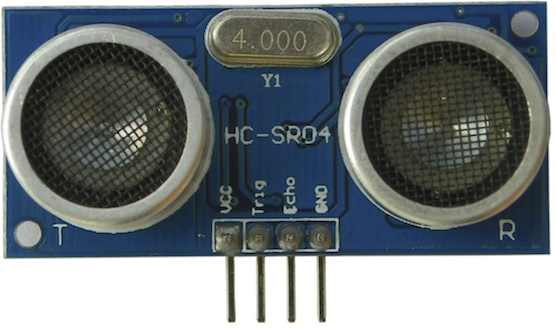
\includegraphics[width=0.3\textwidth]{Billeder/Afstandsmaler/ultra_sensor.png}
\caption{HC-SR04}
\label{fig:HC-SR04}
\end{figure}

\newpage

HC-SR04 aktiveres ved at modtage en trigger puls på minimum 10 \text{µ-sekunder.}
Herefter udsender sensoren 8 burst af 40khz fra sin sender. Efter udsending af de 8 burst sættes echo-benet logisk højt. Når et burst rammer et objekt reflekteres signalet tilbage til HC-SR04 og rammer modtager delen - hvilket sættes echo-benet lavt. Ved at måle pulsbredden på echo-benet kan afstanden udregnes. 

Afstand til objekt kan beregnes på følgende vis: $pulslængde * lydenshastighed * 0.5$

\vspace{0.2cm}

\begin{figure}[H]
\centering
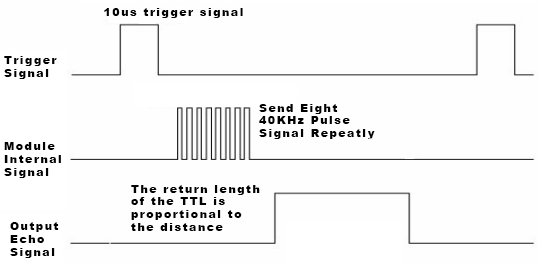
\includegraphics[width=1\textwidth]{Billeder/Afstandsmaler/ultra_schematic.png}
\caption{HC-SR04}
\label{fig:HC-SR04}
\end{figure}

\vspace{2cm}









\section{Kamera}

Under flyvning ønskes det, at der kan tages billeder. Billeder skal sendes til database som systemets bruger kan tilgå. Følgende blev prioriteret højt da der skulle vælges kamera: Kamera skal være kompakt, have lavt strømforbrug og tage billeder med middel opløsning for ikke at bruge så meget båndbredde. 

Til projektet er der overvejet nedenstående tre kamera'er:

\textbf{µCAM} \\
Kameraet der hedder µCAM\footnote{http://www.4dsystems.com.au/downloads/micro-CAM/Docs/uCAM-DS-rev7.pdf} og kan lånes af Ingeniørhøjskolen. Kameraet kan bruges i forskellige modes. Det påregnes, at kameraet skal bruges i det mode hvor der tages billeder i VGA opløsningen. Opløsningen er 640x480 eller 320x240, hvilket passer meget fint med den ønskede opløsning.

\textbf{JPEG Camera adafruit} \\
Dette kamera kan købes på www.adafruit.com\footnote{http://www.adafruit.com/products/1386}. Kameraet er super kompakt og med en vægt på kun 3g. Opløsningen er  640x480 eller 320x240. Til kameraet er der udviklet arduino library til styring af kameraet.

\textbf{FlyCamOne eco V2} \\
Dette kamera kan både optage video og tage billeder. Kameraet kan købes på www.sparkfun.com\footnote{https://www.sparkfun.com/products/11171}. Billede opløsningen er 720x480. Kameraet gemmer film og billeder på et tilhørende SD kort. 

COOKING HACKS!!!





\section{Maincontroller}

Til projektet skal bruges en microcontroller som skal håndtere følgende opgaver:  
\begin{itemize}
	\item Linklag mellem 3G modul og flight control board
	\item Processering af billeder og evt. komprimering.
	\item Læsning fra de forskellige sensorer.
	\item Beregne dronens næste handling. 
	\begin{itemize}
		\item Ud fra nuværende position og ønsket position.
		\item Sørge for at ændre orientering på drone. 
	\end{itemize}
\end{itemize}

\vspace{0.5cm}

Microcontrolleren skal kunne håndtere C++ kode, da det ønskes at programmere objekt orienteret. C++ giver et højt abstraktionsniveau og gør det muligt at bruge klasser og objekter. Dette giver en bedre kodestruktur og gør koden nærmere at overskue.

Desuden skal mircocontrolleren være kompatibel med det 3G-shield der er beskrevet i afsnittet \textit{3G/GPS shield}. 

Både Raspberry Pi og Arduino kan håndtere C++ og er kompatible med 3G-shieldet. Raspberry Pi og Arduino microcontrollere ens på mange punkter. Dog har Raspberry Pi en noget kraftigere processor og besidder nogle unødvendige funktioner. 

Det blev besluttet at bruge et Arduino 2560 board\footnote{http://arduino.cc/en/Main/arduinoBoardMega2560}. Hovedsageligt blev denne microcontroller valgt, da Raspberry Pi krævede en form for mellemlags board og fordi det var muligt at låne Arduino 2560 af Ingeniørhøjskolen. 

\vspace{0.5cm}

\begin{figure}[H]
\centering
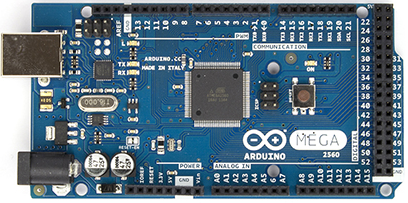
\includegraphics[width=0.5\textwidth]{Billeder/ArduinoMega2560.png}
\caption{Arduino 2560}
\label{fig:Arduino_2560}
\end{figure}



\chapter{Udviklingsværktøjer}

\subsection*{Versions styring}
I overvejelser omkrig værktøjer til versions styring blev kontrol og frihed prioriteret højt. Specielt blev mulighed for selv at styre server og nem oprettelse af nyt repository eller redigering af gamle repository's prioriteret højt.
Det blev besluttet at bruge enten SVN eller GIT. Begge er to meget gode versions styrings værktøjer, der bidrager til god struktur og giver overblink over de dokumenter der udarbejdes og deles. 


\textbf{SVN} \\
SVN er det ældste versions styrings værktøj og er generelt det værktøj der bruges når projekter udarbejdes på Ingeniørhøjskolen. Det betyder at alle gruppens medlemmer har arbejdet med SVN og derved har kendskab til værktøjets stærke og svage sider. 
Desværre opstår der ofte problemer med SVN, da værktøjet i nogle tilfælde er dårligt til at merge filer, hvilket leder til mange merge conflicts. Disse conflicts er tidskrævende og danner grundlag for megen frustration. 

\textbf{GIT} \\
GIT er et nyere versions styrings værktøj og er derfor ikke så vel dokumenteret.
Men GIT er et meget populært værktøj, specielt inden for startup virksomheder, mindre virksomheder og open source projekter. 
En af grundene til GIT er et populært værktøj er, at der findes et hav mange gratis hosting sites, fx. www.github.com. På dette site kan man gratis kan oprette repositoryies og derefter let kan dele det. 
En anden grund til GIT's store popularitet er måden hvorpå GIT håndtere versions styring. I stedet for at skulle pushe alt til serveren og derefter merge det hele på serveren, har hvert gruppemedlem deres eget repository på deres computer og gruppen har et fælles på deres server. Dette muliggøre offline arbejde og meget bedre merge kontrol. \\

Det blev besluttet at bruge GIT, da GIT er gratis og stor kontrol og frihed.
\subsection*{Integrations test - Jenkins}
Jenkins er et værktøj som vi har valgt at intrigere i vores udvikling. Jenkins er en integrations server som hele tiden overvåger vores repository og hver gang der bliver commitet nyt kode der til, så tager Jenkins vores projekt og bygger det samt alle vores software tests vi har skrevet der til. Dette er med til at sikre en meget høj kode standart og give et meget godt overblik over processen i arbejdsforløbet.  
\subsection*{Programmeringssprog}

\textbf{{\LARGE Arduino}} \\
Arduino er et opensource miljø som kan køre helt uafhængigt af OS. Sproget på arduino er en blanding af C og C++ alt afhængigt af hvor hardware nær koden skal være. \newline

\textbf{{\LARGE Server}} \\
Omkrig server delen af projektet havde vi nogle overvejelser. Blandt andet blev læsbarhed, testbar og strukturering blev prioriteret højt da sprog og framework skulle findes. Nedenfor er lavet en beskrivelse af de 3 muligheder der blev overvejet. \newline

\textbf{PHP}\\
PHP er et scripting sprog til serverside programmering. Læringskurven er meget lav og sproget er meget fleksibelt. Da det er et scripting sprog, er det ikke muligt at lave objekt orientering programmering. Med PHP udvikling ville vi gå meget på kompromis med strukturering for fleksibilitet. 

\textbf{Ruby} \\
Ruby og Ruby On Rails er et forhåndsvist nyt udviklings værktøj/sprog til server udvikling. Læringskurven er middel og sproget er tildels fleksibelt. Med Ruby On Rails er det muligt at skrive alt koden objekt orienteret. Sproget er tildels testbart, men det er dog ikke fokus i sproget. 

\textbf{Python} \\
Python er et ældre programmerings sprog, som er kendt for sin stramme syntaks. Pga. den stramme syntaks er læringskurven stejlere end hos de to andre sprog.
Python bliver i modsætning til PHP og Ruby bliver brugt til meget andet end web udvikling, derfor er test frameworket meget stort. Kombineres Python med Django, som er et web-framework - fås et stort og meget stabilt test framework. \newline

Både django og ruby on rails er to meget agile frameworks som begge benytter sig af Model view controller modellen, hvilket er ideelt. Men da gruppens medlemmer allerede besad lidt kendskab til python og pythons gode test framework, blev python + django valgt som sprog og framework til server arbejdet.

\newpage

\textbf{Udvidet test framework} \\
I samarbejde med python og django test frameworket har gruppen også valgt at inddrage Selenium teknologien. Selenium er et værktøj som kan automatisere en browser, dvs. der kan skrives kode som så kan teste GUI'et og selve funktionaliteten i webapplikationen. 

\textbf{Database}\\
Django frameworket understøtter en række forskellige databaser. Det er valgt at benytte en SQLight database, da dette er en simpel light weight database og dækker applikations behov for at kunne gemme billeder og tekst strenge. 
\section{IDE}

\textbf{Arduino} \\
For at kunne udvikle kode til arduinoen, kræver det et IDE. Arduino har lavet deres eget IDE, der indeholder alle de nødvendige biblioteker og funktionalitet der skal til for at skrive kode. Men arduino IDE'et er ikke designet til større projekter, og det er derfor tiltænkt at anvende et andet IDE til projektet. 
Igennem undervisningen på IHA er der blevet stiftet bekendskab med Atmel Studio og Eclipse. \\

\textbf{Atmel Studio} \\
Atmel Studio er valgt som programmerings IDE til dronen. Dette er sket på baggrund af, at Atmel Studio er udviklet til at programmere arduinoer og andre micro controllere. \\

\textbf{Eclipse} \\
Eclipse er et IDE der er designet til højniveaus programmering. Eclipse har ligesom Atmel mulighed for at tilføje eksterne biblioteker, hvilket gør udvigelsen med Arduino simpel. \\

\textbf{Server} \\
Server programmeringen og python koden vil blive udviklet i en tekst editor, Atom.  

\section{Server opsætning}
Serveren udvikles som en RESTful applikation. Som sender/modtager data fra/til dronen.

\subparagraph*{Kommunikation}
Serveren og dronen kommunikere via http-protokollen. Ved brug af GET og POST requests kan vi sende data frem og tilbage imellem serveren og dronen.

\subparagraph*{GUI}
Til håndteringen af designet på GUIet vil Bootstrap frameworket blive benyttet. Hvilket giver en masse gode og flotte design muligheder. 



%%%% Kilder %%%%
\begingroup
\raggedright
\bibliography{bibtex/litteratur}							
% Litteraturlisten inkluderes
\endgroup

%%%% Fixme-listen %%%%
\newpage														% Ny side til Fixme-listen
%\listoffixmes													% Fixme-listen - fjernes til sidst i projektet med "%"

%%%% Appendiks %%%%
\appendix														% Appendiks/bilag start - giver chapter bogstaver i stedet for tal
\clearforchapter												% Sikrer at pagestylen aktiveres paa den rigtige side
\phantomsection													% Kunstigt afsnit, som hyperlinks kan 'holde fast i'
\pdfbookmark[0]{Appendiks}{appendiks}							% Tildeler en klikbar bookmark til den endelige PDF

\end{document}													% Slutter dokumentet - obligatorisk